\documentclass{article}

\usepackage{graphicx}
\usepackage{tikz}
\usepackage{tikzsymbols}
\usetikzlibrary{calc,patterns,shapes.geometric}
\pagestyle{empty}
\usepackage[margin=0pt]{geometry}
\geometry{papersize={14in,12in}}

\def\centerarc[#1](#2)(#3:#4:#5){\draw[#1] ($(#2)+({#5*cos(#3)},{#5*sin(#3)})$) arc (#3:#4:#5);}

\begin{document}
	\begin{figure}
		\centering
		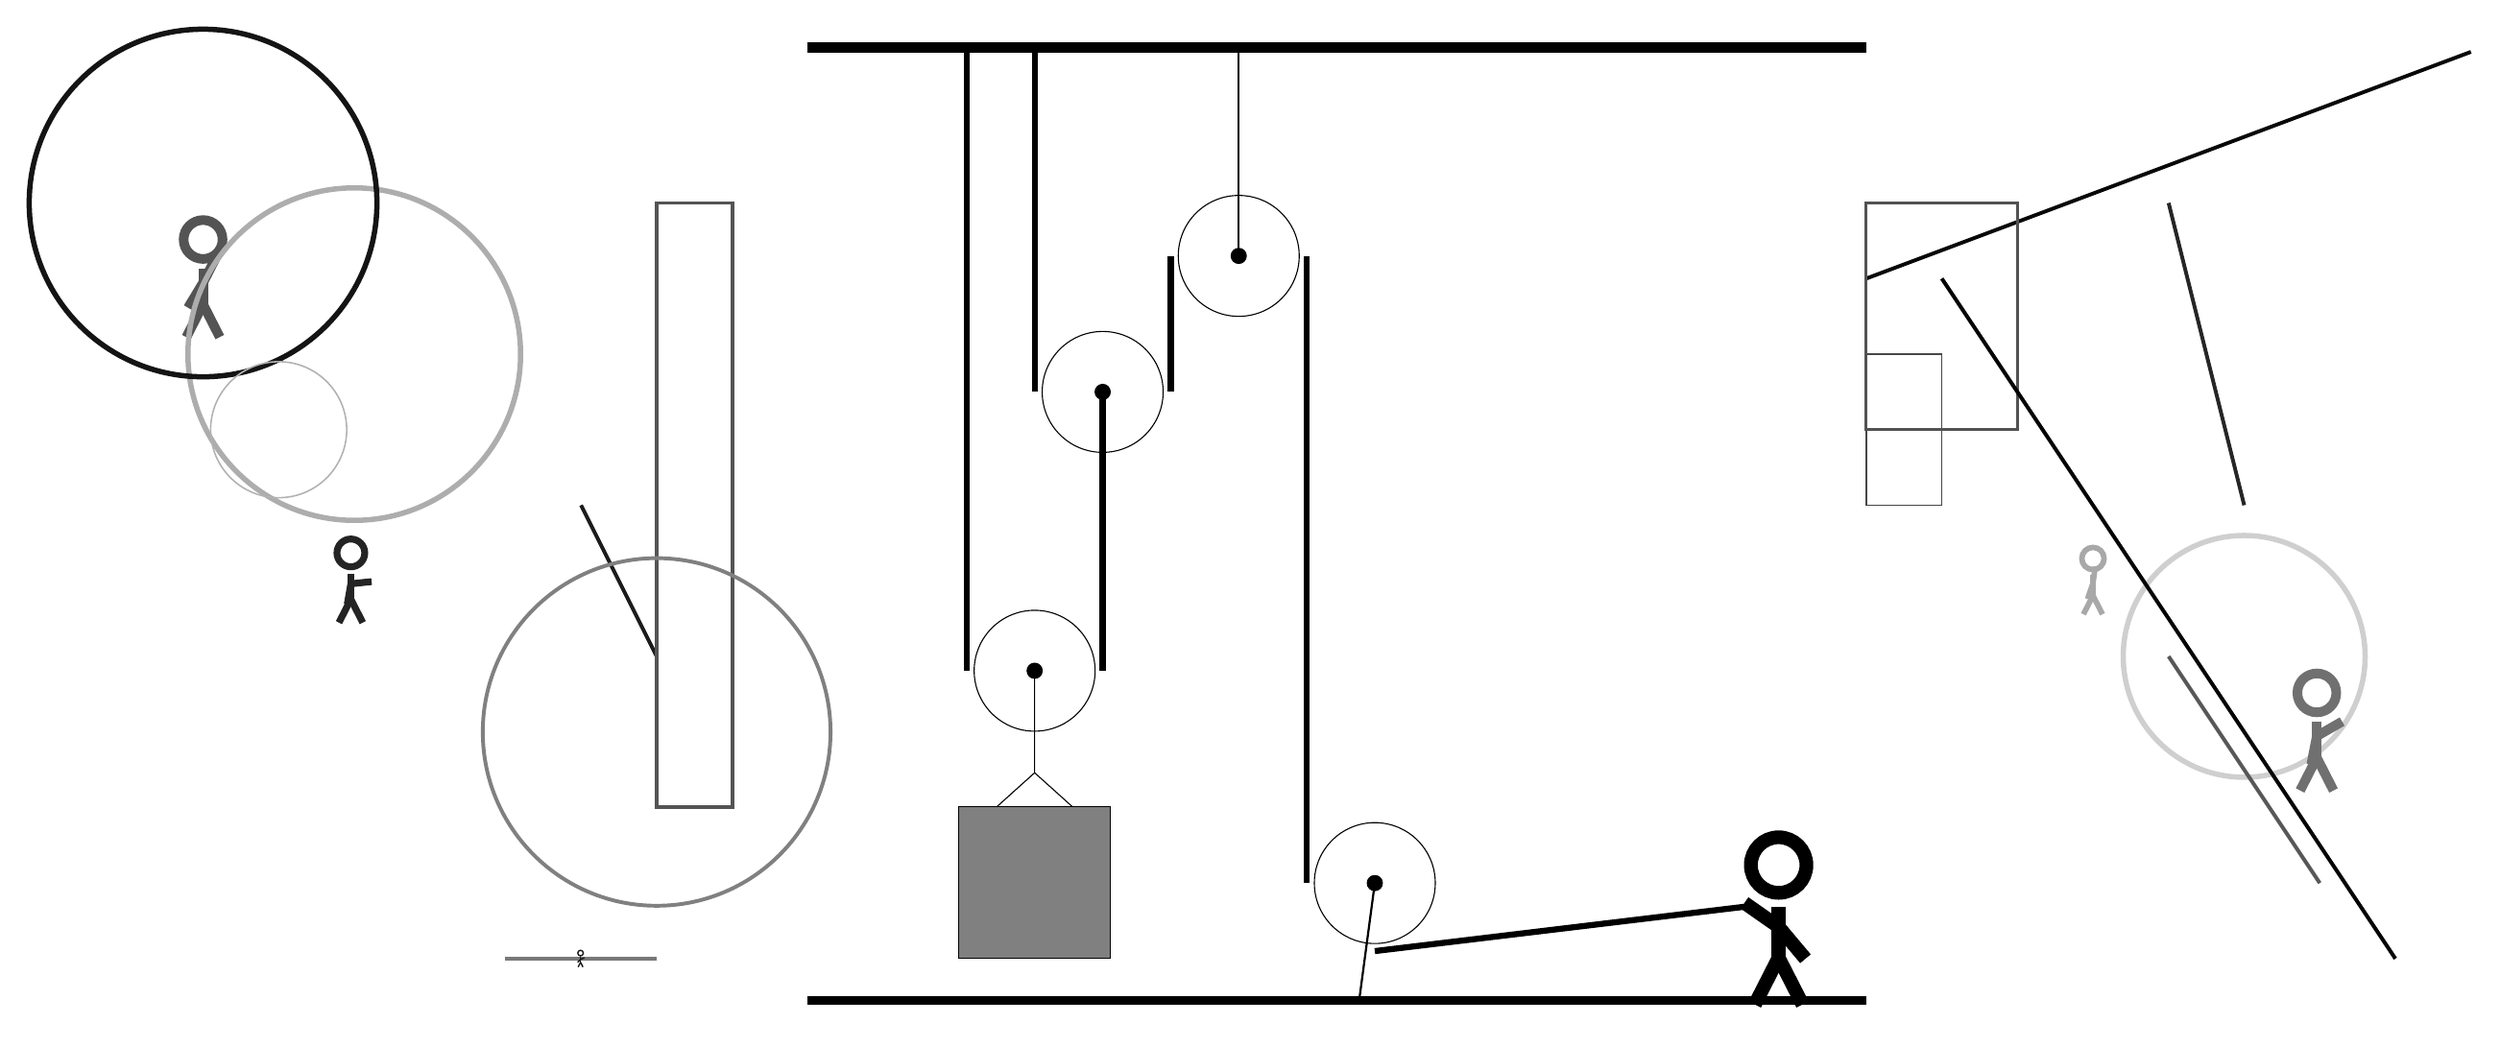
\begin{tikzpicture}
			%%%%% START %%%%%
			
			\draw[fill=black] (-2, 9) rectangle (12, 9.125);
			
			\draw (1, 0.81) circle (0.8);
			\draw[fill=black] (1, 0.81) circle (0.1);
			
			\draw (1.9, 4.5) circle (0.8);
			\draw[fill=black] (1.9, 4.5) circle (0.1);
			
			\draw (3.7, 6.3) circle (0.8);
			\draw[fill=black] (3.7, 6.3) circle (0.1);
			\draw[thick] (3.7, 6.3) -- (3.7, 9);
			
			\draw (5.5, -2) circle (0.8);
			\draw[fill=black] (5.5, -2) circle (0.1);
			\draw[thick] (5.5, -2) -- (5.3, -3.5);
			
			\draw (1, 0.81) -- (1, -0.54) -- (0.5, -0.99) -- (1.5, -0.99) -- (1, -0.54);
			\draw[fill=black!50] (0, -0.99) rectangle (2, -2.99);
			\draw[line width=0.8mm] (0.1, 9) -- (0.1, 0.81);
			\centerarc[line width=0.8mm](1, 0.81)(180:360:0.9);
			\draw[line width=0.8mm](1.9, 0.81) -- (1.9, 4.5);
			\draw[line width=0.8mm] (1.0, 9) -- (1.0, 4.5);
			\centerarc[line width=0.8mm](1.9, 4.5)(180:360:0.9);
			\draw[line width=0.8mm](2.8, 4.5) -- (2.8, 6.3);
			\centerarc[line width=0.8mm](3.7, 6.3)(0:180:0.9);
			\draw[line width=0.8mm] (4.6, 6.3) -- (4.6, -2);
			\centerarc[line width=0.8mm](5.5, -2)(0:90:-0.9);
			\draw[line width=0.8mm](5.5, -2.9) -- (10.5, -2.3);
			
			\node at (10.8, -2.5) {\Strichmaxerl[10][-35][-50]};
			
			\draw[line width=0.2mm, color=black!72] (13, 5) rectangle (12, 3);
			
			\node[line width=0.7mm, color=black!67] at (-10, 6) {\Strichmaxerl[7][59][63]};
			\node[line width=0.6mm, color=black!34] at (15, 2) {\Strichmaxerl[4][71][82]};
			\draw[line width=0.5mm, color=black!89](-5, 3) -- (-4, 1);
			\draw[line width=0.5mm, color=black!85](17, 3) -- (16, 7);
			\draw [line width=0.7mm, color=black!19](17, 1) circle (1.6);
			
			\draw[line width=0.5mm, color=black!97](12, 6) -- (20, 9);
			\draw[line width=0.5mm, color=black!67] (-4, 7) rectangle (-3, -1);
			\draw[line width=0.5mm, color=black!66](16, 1) -- (18, -2);
			
			\node[line width=0.7mm, color=black!86] at (-8, 2) {\Strichmaxerl[5][80][6]};
			\draw[line width=0.4mm, color=black!68] (14, 4) rectangle (12, 7);
			\draw [line width=0.7mm, color=black!32](-8, 5) circle (2.2);
			\draw[line width=0.5mm, color=black!99](13, 6) -- (19, -3);
			
			\node[line width=0.5mm, color=black!56] at (18, 0) {\Strichmaxerl[7][79][30]};
			\draw[line width=0.5mm, color=black!53](-6, -3) -- (-4, -3);
			\draw [line width=0.5mm, color=black!50](-4, 0) circle (2.3);
			
			\node[line width=0.7mm, color=black!90] at (-5, -3) {\Strichmaxerl[1][46][20]};
			\draw [line width=0.7mm, color=black!92](-10, 7) circle (2.3);
			\draw [line width=0.2mm, color=black!30](-9, 4) circle (0.9);
			
			\draw[fill=black] (-2, -3.5) rectangle (12, -3.6);
			
			%%%%% END %%%%%
		\end{tikzpicture}
	\end{figure}	
\end{document}